%
% This is a borrowed LaTeX template file for lecture notes for CS267,
% Applications of Parallel Computing, UCBerkeley EECS Department.
% Now being used for CMU's 10725 Fall 2012 Optimization course
% taught by Geoff Gordon and Ryan Tibshirani.  When preparing 
% LaTeX notes for this class, please use this template.
%
% To familiarize yourself with this template, the body contains
% some examples of its use.  Look them over.  Then you can
% run LaTeX on this file.  After you have LaTeXed this file then
% you can look over the result either by printing it out with
% dvips or using xdvi. "pdflatex template.tex" should also work.
%

\documentclass[twoside]{article}
\setlength{\oddsidemargin}{0.25 in}
\setlength{\evensidemargin}{-0.25 in}
\setlength{\topmargin}{-0.6 in}
\setlength{\textwidth}{6.5 in}
\setlength{\textheight}{8.5 in}
\setlength{\headsep}{0.75 in}
\setlength{\parindent}{0 in}
\setlength{\parskip}{0.1 in}

%
% ADD PACKAGES here:
%

\usepackage{amsmath,amsfonts,graphicx}

%
% The following commands set up the lecnum (lecture number)
% counter and make various numbering schemes work relative
% to the lecture number.
%
\newcounter{lecnum}
\renewcommand{\thepage}{\thelecnum-\arabic{page}}
\renewcommand{\thesection}{\thelecnum.\arabic{section}}
\renewcommand{\theequation}{\thelecnum.\arabic{equation}}
\renewcommand{\thefigure}{\thelecnum.\arabic{figure}}
\renewcommand{\thetable}{\thelecnum.\arabic{table}}

%
% The following macro is used to generate the header.
%
\newcommand{\lecture}[4]{
   \pagestyle{myheadings}
   \thispagestyle{plain}
   \newpage
   \setcounter{lecnum}{#1}
   \setcounter{page}{1}
   \noindent
   \begin{center}
   \framebox{
      \vbox{\vspace{2mm}
    \hbox to 6.28in { {\bf EE302 - Feedback Systems
	\hfill Spring 2019} }
       \vspace{4mm}
       \hbox to 6.28in { {\Large \hfill Lecture #1 \hfill} }
       \vspace{2mm}
       \hbox to 6.28in { {\it Lecturer: #2 \hfill } }
      \vspace{2mm}}
   }
   \end{center}
   \markboth{Lecture #1}{Lecture #1}

   \vspace*{4mm}
}
%
% Convention for citations is authors' initials followed by the year.
% For example, to cite a paper by Leighton and Maggs you would type
% \cite{LM89}, and to cite a paper by Strassen you would type \cite{S69}.
% (To avoid bibliography problems, for now we redefine the \cite command.)
% Also commands that create a suitable format for the reference list.
\renewcommand{\cite}[1]{[#1]}
\def\beginrefs{\begin{list}%
        {[\arabic{equation}]}{\usecounter{equation}
         \setlength{\leftmargin}{2.0truecm}\setlength{\labelsep}{0.4truecm}%
         \setlength{\labelwidth}{1.6truecm}}}
\def\endrefs{\end{list}}
\def\bibentry#1{\item[\hbox{[#1]}]}

%Use this command for a figure; it puts a figure in wherever you want it.
%usage: \fig{NUMBER}{SPACE-IN-INCHES}{CAPTION}
\newcommand{\fig}[3]{
			\vspace{#2}
			\begin{center}
			Figure \thelecnum.#1:~#3
			\end{center}
	}
% Use these for theorems, lemmas, proofs, etc.
\newtheorem{theorem}{Theorem}[lecnum]
\newtheorem{lemma}[theorem]{Lemma}
\newtheorem{proposition}[theorem]{Proposition}
\newtheorem{claim}[theorem]{Claim}
\newtheorem{corollary}[theorem]{Corollary}
\newtheorem{definition}[theorem]{Definition}
\newenvironment{proof}{{\bf Proof:}}{\hfill\rule{2mm}{2mm}}

% **** IF YOU WANT TO DEFINE ADDITIONAL MACROS FOR YOURSELF, PUT THEM HERE:

\begin{document}

% Lecture Details
\lecture{11}{Asst. Prof. M. Mert Ankarali}

\par 

\section{Stability}

A SISO system is called BIBO (bounded-input--bounded-output) stable,
if the output will be bounded for \textbf{every} input to the system that is
bounded. 

  \begin{minipage}[h]{1\linewidth}
    \begin{center}
      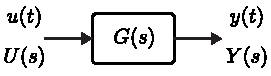
\includegraphics[width=0.5\textwidth]{sys}
    \end{center}
  \end{minipage}
 
If we use the impulse response representation for an LTI SISO system, i.e.. $y(t) =
\int_{0}^{t} g(t) u(t - \tau) d \tau$ (we assume that system is causal),
the system is BIBO stable if and only if its impulse response is 
absolutely integrable.
%
\begin{align*}
   \mathrm{BIBO} \ \mathrm{Stable} \ \Leftrightarrow \ \int_0^{\infty } |
  g(t) | dt < B < \infty
\end{align*}
 %
However, we genrally use transfer function representation in this
course. Let 
%
\begin{align*}
  \frac{Y(s)}{U(s)} =  G(s) = \frac{N(s)}{D(s)}
\end{align*}
%
In this context, a rational transfer function representation is BIBO stable if and only if, 
 the poles of $G(s)$ (or roots of $D(s)$ ) are strictly located  in
 the open left half $s-$plane.

\textbf{Ex:} Show that $G(s) = \frac{1}{s}$ is not BIBO stable

\textbf{Solution:} Let's first check the impulse response condition
%
\begin{align*}
  g(t) &= 1 , \ t \geq 0
  \\
  \lim_{t \to \infty} \int_{0}^{t} | g(\tau) | d \tau &= \lim_{t \to \infty}
  \int_{0}^{t} 1 d \tau = \infty 
\end{align*}
%
Thus the system is BIBO unstable. The system has a single pole at the
origin, so we already know that it is BIBO unstable. Now, let's 
find a specific bounded input such that output is unbounded.
Let $u(t)$ be the unit-step input then
%
\begin{align*}
   Y(s) &= \frac{1}{s^2} \ \Rightarrow \ y(t) = t  \ , t \geq 0
\\
 \lim_{t \to \infty} | y(t) | &= \infty
\end{align*}
%
Obviously, we obtained an un-bounded output.

\textbf{Ex:} Let $G(s) = \frac{1}{s^2 + 1}$. Find a
bounded input, such that output is unbounded.
%
\textbf{Solution:} Let $u(t) = \cos t \ , t \geq 0$, then
%
\begin{align*}
  Y(s) &= G(s) U(s) = \frac{s}{(s^2+1)^2}
  \\
  y(t) &= t \sin t \ , t \geq > 0
\end{align*}
%
Now we obtain an un-bounded output due to the resonance effect. 

\subsection{Stability of First \& Second Order Systems}

In order to gain some intuition about how to check stability
of general rational LTI systems, we will analyze first and second order
systems. 

The transfer function of a first order system has the form
%
\begin{align*}
  D(s) &= a_0 s + a_1 \\
 a_0 &> 0 , \ \mathrm{w.l.g}
\end{align*}
%
The single pole of the system and associated stability condition 
can be derived as
%
\begin{align*}
  p &= -\frac{a_1}{a_0}
 \\
  \mathrm{Stable} &\Leftrightarrow a_1 > 0
\end{align*}

Now lets analyze second order systems. Transfer function
of a second order system has the following form
%
\begin{align*}
  D(s) &= a_0 s^2 + a_1 s + a_2\\
 a_0 &> 0 , \ \mathrm{w.l.g}
\end{align*}
%
If we carefully analyze $\mathrm{Sign} [ D(0 ]$, 
we can see that
%
\begin{itemize}
     \item $\mathrm{Sign} [ D(0) ] < 0$, one pole is located in the
       open-left half plane, where as the other one is located in the
       open- right half plane.
     \item $\mathrm{Sign} [ D(0) ] = 0$, there exist at least one pole 
     at the origin.
\end{itemize}
%
In this context, we can derive the first condition (necessary but not
sufficient) 
%
\begin{align*}
 \mathrm{Stable} \Rightarrow a_2 > 0 
\end{align*}
%
Under this condition, we can re-write the characteristic
equation in a more standard form
%
\begin{align*}
  &D(s) = a_0 \left( s^2 + \frac{a_1}{a_0} s + \frac{a_2}{a_0} \right)
  \\
  &D(s) = a_0 \left( s^2 + 2 \zeta \omega_n s + \omega_n^2 \right)
  \\
  &\mathrm{where}
\\
 &\omega_n = \sqrt{a_2 / a_0} > 0 
\\
  &\zeta = \frac{a_1}{2 a_0 \omega_n} 
\end{align*}
%
From the analysis of second order system in standard form,
we know that when 
%
\begin{itemize}
  \item $\zeta < 0$, system poles are located in the open right-half
    plane
  \item $\zeta = 0$, system poles are located on the imaginary axis
  \item $\zeta > 0$, system poles are located in the open left-half
    plane
\end{itemize}
%
It is also easy to see that $\zeta > 0 \Leftrightarrow a_1 > 0$. 
As a result, we can derive a necessary and sufficient condition on
BIBO stability. 

A second order system with $D(s) = a_o s^2 + a_1 s + a_2$ (with $a_0 >
0$), is BIBO stable if and only if $a_i > 0, \ \forall i \in \lbrace 1
, 2 \rbrace$.

\subsection{Routh's Stability Criterion} 

Routh's Stability Criterion (a.k.a  Routh–Hurwitz stability criterion)
is a mathematical test that is a necessary and sufficient condition 
for the stability of an LTI system. The Routh test is a very 
computationally efficient algorithm for the test of absolute
LTI system stability. 

In this test, one first constructs the routh table for a given
%
\begin{align*}
D(s) = a_o s^n + a_1 s^{n-1} + a_2 s^{n-3} + \cdots + a_{n-2} s^{2}
+ a_{n-1} s^{1} + a_n 
\end{align*}  
%
which has $n+1$ rows. 
%
\begin{table}[h]
\begin{center}
\begin{tabular}{|c || c || c c c c |}
\hline
$s^n$ & $a_0$ & $a_2$ & $a_4$ & $a_6$ & $\cdots$ 
\\ \hline
$s^{n-1}$ & $a_1$ & $a_3$ & $a_5$ & $a_7$ & $\cdots$ 
\\ \hline
$s^{n-2}$ & $b_1$ & $b_2$ & $b_3$ & $b_4$ & $\cdots$ 
\\ \hline
$s^{n-3}$ & $c_1$ & $c_2$ & $c_3$ & $c_4$ & $\cdots$ 
\\ \hline
$s^{n-4}$ & $d_1$ & $d_2$ & $d_3$ & $d_4$ & $\cdots$ 
\\ \hline
$\vdots$ & $\vdots$ & $\vdots$ &  & & 
\\ \hline
$s^{2}$ & $e_1$ & $e_2$ & $0$ & $\cdots$  & 
\\ \hline
$s^{1}$ & $f_1$ & $0$ & $0$ & $\cdots$  & 
\\ \hline
$s^{0}$ & $g_0$ & $0$ & $0$ & $\cdots$  & 
\\ \hline
\end{tabular}
\end{center}
\end{table}

where the coefficents $b_i$ are computed with
%
\begin{align*}
 b_1 = - \mathrm{det}\left( \left[ \begin{array}{cc} a_0 & a_2 \\ a_1
                                                         &
                                                           a_3 \end{array}
                                                           \right]
                                                           \right) / a_1
=
\frac{a_1 a_2 - a_0 a_3 }{a_1}
\\
b_2 = - \mathrm{det}\left( \left[ \begin{array}{cc} a_0 & a_4 \\ a_1
                                                         &
                                                           a_5 \end{array}
                                                           \right]
                                                           \right) / a_1
=
\frac{a_1 a_4 - a_0 a_5 }{a_1}
\\
b_3 = - \mathrm{det}\left( \left[ \begin{array}{cc} a_0 & a_6 \\ a_1
                                                         &
                                                           a_7 \end{array}
                                                           \right]
                                                           \right) / a_1
=
\frac{a_1 a_6 - a_0 a_7 }{a_1}
\\
\vdots
\end{align*}  
%
coefficents $c_i$ are computed with
%
%
\begin{align*}
& c_1 = - \mathrm{det}\left( \left[ \begin{array}{cc} a_1 & b_1 \\ a_3
                                                         &
                                                           b_2 \end{array}
                                                           \right]
                                                           \right) / b_1
=
\frac{b_1 a_3 - a_1 b_2 }{b_1}
\\
&c_2 = - \mathrm{det}\left( \left[ \begin{array}{cc} a_1 & a_5 \\ b_1
                                                         &
                                                           b_3 \end{array}
                                                           \right]
                                                           \right) / b_1
=
\frac{b_1 a_5 - a_1 b_3 }{b_1}
\\
&c_3 = - \mathrm{det}\left( \left[ \begin{array}{cc} a_1 & a_7 \\ b_1
                                                         &
                                                           b_4 \end{array}
                                                           \right]
                                                           \right) / b_1
=
\frac{b_1 a_7 - a_1 b_4 }{b_1}
\\
&\vdots
\end{align*}  

Coefficents $d_i$ are computed with
%
\begin{align*}
& d_1 = - \mathrm{det}\left( \left[ \begin{array}{cc} b_1 & b_2 \\ 
                                      c_1 & c_2 \end{array}
                                                           \right]
                                                           \right) /c_1
=
\frac{c_1 b_2 - b_1 b_2 }{c_1}
\\
&d_2 = - \mathrm{det}\left( \left[ \begin{array}{cc} b_1 & b_3 \\ c_1
                                                         &
                                                           c_3 \end{array}
                                                           \right]
                                                           \right) / c_1
=
\frac{c_1 b_3 - b_1 c_3 }{c_1}
\\
&d_3 = - \mathrm{det}\left( \left[ \begin{array}{cc} b_1 & b_4 \\ c_1
                                                         &
                                                           c_4 \end{array}
                                                           \right]
                                                           \right) / c_1
=
\frac{c_1 b_4 - b_1 c_4 }{c_1}
\\
&\vdots
\end{align*}  
%
Other coefficients are computed with the same structure with the
computation flow of $d_i$'s. 

\textbf{Result 1:} The system is NOT BIBO stable if $\exists \, i , \ s.t ,\
a_i \leq 0 $. In other words, since we assumed $a_0 > 0$, all other
coefficients have to be strictly positive. This is a necessary, but
not sufficient condition. 

\textbf{Result 2:} The system is BIBO stable, if and only if all the 
coefficients in the first row strictly positive. Routh test provides
a necessary and sufficient condition.  

\textbf{Result 3:} The $\#$ of roots of D(s) with positive real parts 
is equal to the $\#$ of sign changes in the first column (shown in
table below) of the Routh array. 
%
\begin{table}[h]
\begin{center}
\begin{tabular}{|| c || }
\hline
$a_0$ 
\\ \hline
$a_1$ 
\\ \hline
$b_1$ 
\\ \hline
$c_1$ 
\\ \hline
$d_1$ 
\\ \hline
$\vdots$ 
\\ \hline
$e_1$ 
\\ \hline
$f_1$ 
\\ \hline
$g_0$ 
\\ \hline
\end{tabular}
\end{center}
\end{table}

\textbf{Ex:} Let $D(s) = s^4 + 2 s^3 + 3 s^2 + 4 s + 5$, is this
system is stable. If not what is the number of poles with positive 
real parts. 

\textbf{Solution:} Let's build the Routh table

\begin{minipage}[h]{1\linewidth}
\begin{center}
\begin{tabular}{|c || c || c c c |}
\hline
$s^4$ & 1 & 3 & 5 & 0 
\\ \hline
$s^3$ & 2 & 4 & 0 & 0 
\\ \hline
$s^2$ & $\frac{2 \cdot 3 - 1 \cdot 4}{2} = 1$ & $\frac{2 \cdot 5 - 1 \cdot 0}{2} = 5$  & 0 & 0
\\ \hline
$s^1$ &  $\frac{1 \cdot 4 - 2 \cdot 5}{1} = -6$ & 0 & 0 & 0 
\\ \hline
$s^0$ & 5 & 0 & 0 & 0 
\\ \hline
\end{tabular}
\end{center}
\end{minipage}

\vspace{6pt}

$\#$ sign changes is equal to $2$, thus the system is unstable and 2
out of 4 poles are located in the open right-half plane. If we
compute the poles numerically using a programming environment, 
we can find that $p_{1,2} =   -1.29 \pm 0.86 j$ and  $p_{3,4} = 0.29
\pm 1.4 j$, which indeed verifies the Routh table result. 
 
\vspace{12pt}

\textbf{Ex:} Consider the following closed-loop system, find 
the set of $K_P$ and $K_D$ gains such that closed-loop system is stable

  \begin{minipage}[h]{1\linewidth}
    \begin{center}
      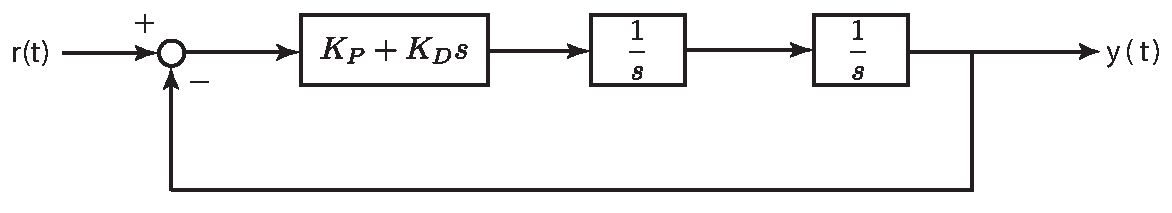
\includegraphics[width=0.75\textwidth]{example2}
    \end{center}
  \end{minipage}

\textbf{Solution:} Denominator of the closed-loop transfer function 
of the system has the following form
$D(s) = s^2 + K_D s + K_P$. Now, lets construct the Routh table for the $D(s)$
%
\begin{table}[h]
\begin{center}
\begin{tabular}{|c || c || c  |}
\hline
$s^2$ & 1 & $K_P$ 
\\ \hline
$s^1$ & $K_D$ & 0 
\\ \hline
$s^0$ & $K_P$ & 0 
\\ \hline
\end{tabular}
\end{center}
\end{table}

In order the closed-loop system to be stable, $\#$ sign changes in the
first column must
be equal to zero, thus the closed-loop system is BIBO stable
if and only if $K_P > 0$ and $K_D > 0$.

\vspace{6pt} 

\textbf{Ex:} Consider the following closed-loop system, find 
the set of $K_I$ gains such that closed-loop system is stable

  \begin{minipage}[h]{1\linewidth}
    \begin{center}
      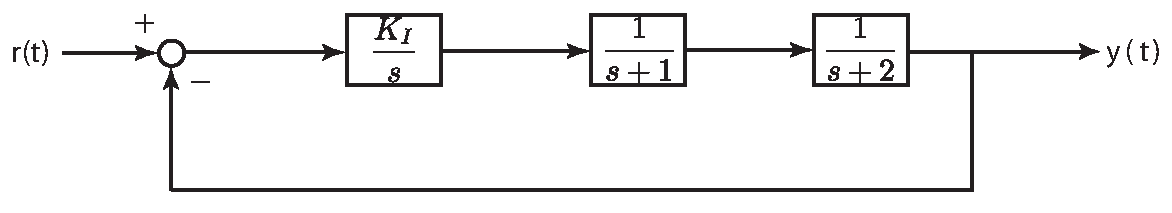
\includegraphics[width=0.75\textwidth]{example5}
    \end{center}
  \end{minipage}

\textbf{Solution:} Denominator of the closed-loop transfer function 
of the system has the following form
%
\begin{align*}
D(s) = s^3 + 3 s^2 + 2 s + K_I 
\end{align*}
%
Now, lets construct the Routh table for the $D(s)$

 \begin{minipage}[h]{1\linewidth}
\begin{center}
\begin{tabular}{|c || c || c  |}
\hline
$s^3$ & 1 & $2$ 
\\ \hline
$s^2$ & 3 & $K_I$ 
\\ \hline
$s^1$ & $\frac{6 - K_I}{3}$ & 0 
\\ \hline
$s^0$ & $K_I$ & 0 
\\ \hline
\end{tabular}
\end{center}
  \end{minipage}

In order the closed-loop system to be stable, $\#$ sign changes in the
first column must be equal to zero, thus the closed-loop system is BIBO stable
if and only if $K_I \in (0 , 6)$.

\subsubsection{Routh Hurwitz Stability Test: Special Cases}

\paragraph{Case I:}

Let's analyze the stability of ``$D(s) = s^3 - 3 s + 2$''. 
Since $a_1 = 0$ and $a_2 = -3$, we know that the system
is not BIBO stable. Let's construct the Routh table to verify this result.

 \begin{minipage}[h]{1\linewidth}
\begin{center}
\begin{tabular}{|c || c || c  |}
\hline
$s^3$ & 1 & $-3$ 
\\ \hline
$s^2$ & 0 & 2
\\ \hline
$s^1$  & ? & 
\\ \hline
$s^0$  & ? & 
\\ \hline
\end{tabular}
\end{center}
  \end{minipage}

We can see that one of the coefficients in the Routh array is zero,
and we can not complete the Rout table. If a coefficient in the Routh
array is zero, we know from the Routh Hurwitz test that the system is
BIBO unstable. However, what can we do, if we want to compute the 
$\#$ poles with positive real parts. 

\vspace{12pt}

\textbf{Solution Type 1:} Lets find a new $\bar{D}(s) = (s + \alpha)
D(s), \ \alpha > 0$. We know that $D(s)$ and $\bar{D}(s)$ has the same 
$\#$ poles with positive real parts. Then we can construct a Routh
table for $\bar{D}(s)$ to seek an answer. 

Let $\bar{D}(s) = (s + 2) ( s^3 - 3 s + 2) = s^4 + 2 s^3 - 3 s^2 - 4 s+ 4$, the Routh table takes the form

%
\begin{table}[h]
\begin{center}
\begin{tabular}{|c || c || c c |}
\hline
$s^4$ & 1 & -3 & 4 
\\ \hline
$s^3$ & 2 & -4 & 0
\\ \hline
$s^2$ & -1 & 4 & 0
\\ \hline
$s^1$ & 4 & 0 &
\\ \hline
$s^0$ & 4 & 0 & 
\\ \hline
\end{tabular}
\end{center}
\end{table}
%
$\#$ sign changes in the Routh array of $\bar{D}(s)$ is equal to 2, so
we can conclude that $D(s)$ has 2 poles with positive real parts. If
we compute the poles of $D(s)$, we find that $p_1 = 2$, $p_{2,3} = 1$,
which verifies our finding. 

\vspace{12pt}

\textbf{Solution Type 2:} Replace 0 element with an infinitesimal but
non-zero element $\epsilon >0$.
%
\begin{table}[h]
\begin{center}
\begin{tabular}{|c || c || c  |}
\hline
$s^3$ & 1 & $-3$ 
\\ \hline
$s^2$ & $\epsilon$ & 2
\\ \hline
$s^1$  & $- \frac{3 \epsilon + 2}{\epsilon}$ & 0 
\\ \hline
$s^0$  & 2 & 
\\ \hline
\end{tabular}
\end{center}
\end{table}

$\#$ sign changes in the perturbed Routh array of $D(s)$ is equal to 2, so
we can conclude that $D(s)$ has 2 poles with positive real parts.

\newpage

\textbf{Solution Type 3:} Replace $s$ with $1/q$
%
\begin{align*}
  D(s)|_{s =1/q} = q^{-3} - 3 q^{-1} + 2 = q^{-3} 
  \left( 2 q^{2} - 3 q^2 + 1 \right)
\end{align*}
%
Now let's define $\bar{D}(q) = q^3 D(s)|_{s =1/q} =  2 q^3 - 3 q^2 +
1$. 
Note that we simply flip the coefficients of $D(s)$
to find the coefficients of $\bar{D}(q)$. It is easy to see that 
if $p_i$ is a pole of $D(s)$, then $1/p_i$ is a pole of $\bar{D}(q)$.
Let $p_i = \sigma + j \omega$, then 
%
\begin{align*}
  \frac{1}{p_i} &= \frac{1}{\sigma + j \omega} = \frac{\sigma - j
  \omega}{\sigma^2 + \omega^2}
\\
&= \frac{\sigma}{\sigma^2 + \omega^2} - j \frac{
  \omega}{\sigma^2 + \omega^2}
\\
\mathrm{Sign} ( \mathrm{Re} \lbrace p_i \rbrace ) &= 
\mathrm{Sign} \left( \mathrm{Re} \left\lbrace \frac{1}{p_i} \right\rbrace \right)
\end{align*}
%
We can see that $D(s)$ and $\bar{D}(q)$ have same number of stable
and unstable poles. Thus, we can perform a Routh Hurwitz test on
$\bar{D}(q)$
%
\begin{table}[h]
\begin{center}
\begin{tabular}{|c || c || c  |}
\hline
$s^3$ & 2 & 0 
\\ \hline
$s^2$ & -3 & 1
\\ \hline
$s^1$  & 2/3 & 0 
\\ \hline
$s^0$  & 1 & 
\\ \hline
\end{tabular}
\end{center}
\end{table}

$\#$ sign changes in the Routh array of $\bar{D}(q)$ is equal to 2, so
we can conclude that $D(s)$ has 2 poles with positive real parts.

\paragraph{Case II:}

\paragraph{Ex:} Analyze the stability of $D(s) = s^4 + 2 s^3 + 2 s^2 +
2 s + 1$ using Routh table

\begin{minipage}[h]{1\linewidth}
\begin{center}
\begin{tabular}{|c || c || c c |}
\hline
$s^4$ & 1 & 2 & 1 
\\ \hline
$s^3$ & 2 & 2 & 0
\\ \hline
$s^2$ & 1 & 1 & 0
\\ \hline
$s^1$ & 0 & 0 &
\\ \hline
$s^0$ & ? & ? & 
\\ \hline
\end{tabular}
\end{center}
\end{minipage}

We can see that one row in Routh table is completely zero. 
Thus we know that system is indeed BIBO stable. However,
what we can do in order to find number of unstable poles. 
This happens when there exists roots of equal magnitude
located radially opposite in $s-$plane, i.e. symmetric
w.r.t origin. These cases are illustrated in the figrue below.

\vspace{6pt}

\begin{minipage}[h]{1\linewidth}
    \begin{center}
      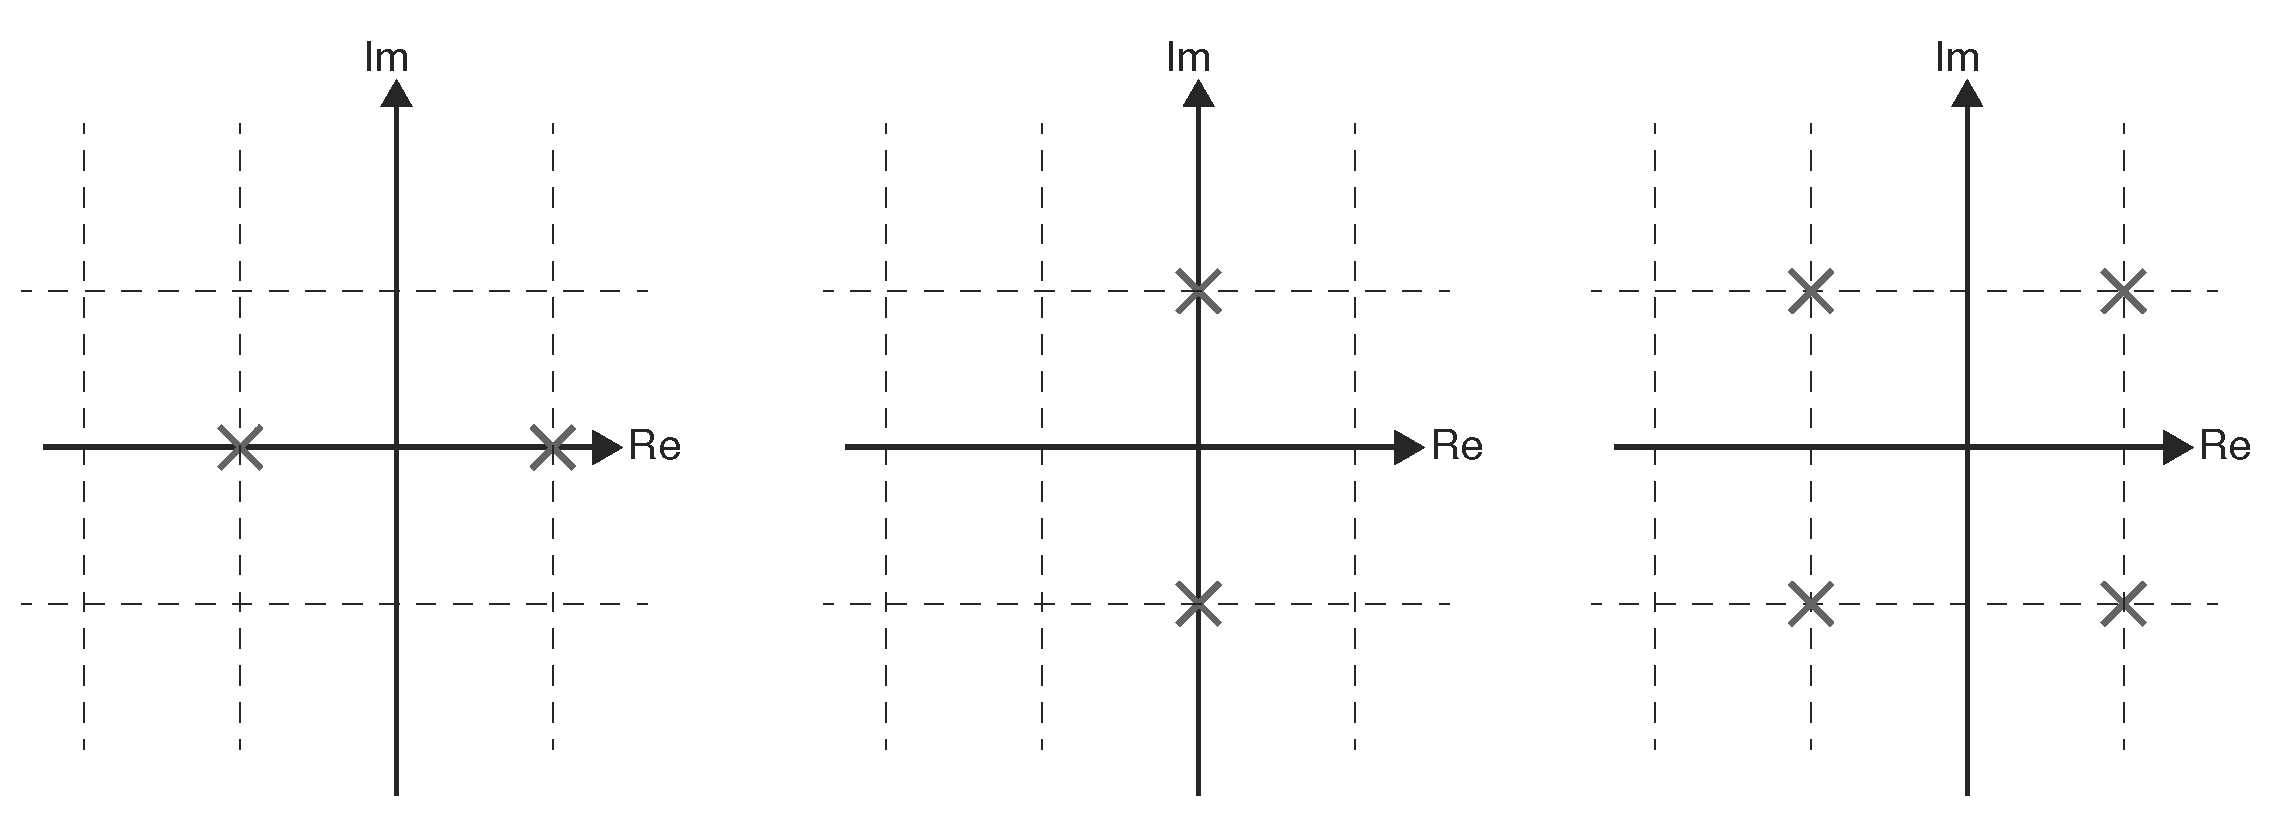
\includegraphics[width=0.95\textwidth]{caseII}
    \end{center}
\end{minipage}

\vspace{6pt}

This case happens always after an even row, in this example right after $s^2$ row. In such 
cases, we compute the Auxiliary polynomial, $A(s) = s^2 + 1$ in this
example. After that, we compute its derivative, $A'(s) = 2 s$ in this example,
and use the coefficient of $A'(s)$ in replacement of the zero row and compute
the Routh array accordingly. This process is illustrated below

\vspace{6pt}
\begin{minipage}[h]{1\linewidth}
\begin{center}
\begin{tabular}{|c || c || c c | l |}
\hline
$s^4$ & 1 & 2 & 1 &
\\ \hline
$s^3$ & 2 & 2 & 0 &
\\ \hline
$s^2$ & 1 & 1 & 0 & $\rightarrow A(s) = s^2 + 1$
\\ \hline
$s^1$ & \textbf{2} & \textbf{0} &   & $\leftarrow A'(s) = 2$
\\ \hline
$s^0$ & 1 & 0 & &
\\ \hline
\end{tabular}
\end{center}
\end{minipage}
\vspace{6pt}

$\#$ sign changes in the Routh array of $D(s)$ with Auxiliary polynomial
is equal to 0, so we can conclude that $D(s)$ has 0 poles with
positive real parts. This means that all unstable poles are located on
the imaginary axis. If we compute the poles numerically we find that
$p_{1,2} = -1$ and $p_{2,3} = - j$ which verifies our finding. Indeed,
we can see that problematic roots are the roots of $A(s)$.

\vspace{6pt}

\textbf{Ex:} Compute $\#$ unstable poles of $D(s) = s^3 + 2 s^2 - s - 2 $ using Routh table
%
\begin{table}[h]
\begin{center}
\begin{tabular}{|c || c || c | l |}
\hline
$s^3$ & 1 & -1 & 
\\ \hline
$s^2$ & 2 & -2 & $\rightarrow A(s) = 2 s^2 - 2$
\\ \hline
$s^1$ & \textbf{2} & \textbf{0} & $\leftarrow A'(s) = 2 s^2 - 2$
\\ \hline
$s^0$ & -2 & 0 & 
\\ \hline
\end{tabular}
\end{center}
\end{table}

$\#$ sign changes in the Routh array of $D(s)$ with Auxiliary polynomial
is equal to 1, so we can conclude that $D(s)$ has 1 pole with
positive real part. If we compute the poles numerically we find that
$p_{1} = -1$, $p_2 = -2$ and $p_{3} = 1$ which verifies our finding. Indeed,
we can see that problematic roots is one of the roots of $A(s)$.

This case occurs when there are roots of equal magnitude lying
radially opposite in the s-plane. 

\newpage

\subsubsection{Routh Hurwitz Stability Test: Relative Stability}

Let's assume that we not only interested in the absolute stability of
a system, but also we would like to test weather all poles are located 
in a region where the real part of the whole poles has an upper bound
of $-4$. Similarly we can think that, we define a performance region
based on a settling time requirement. 

  \begin{minipage}[h]{1\linewidth}
    \begin{center}
      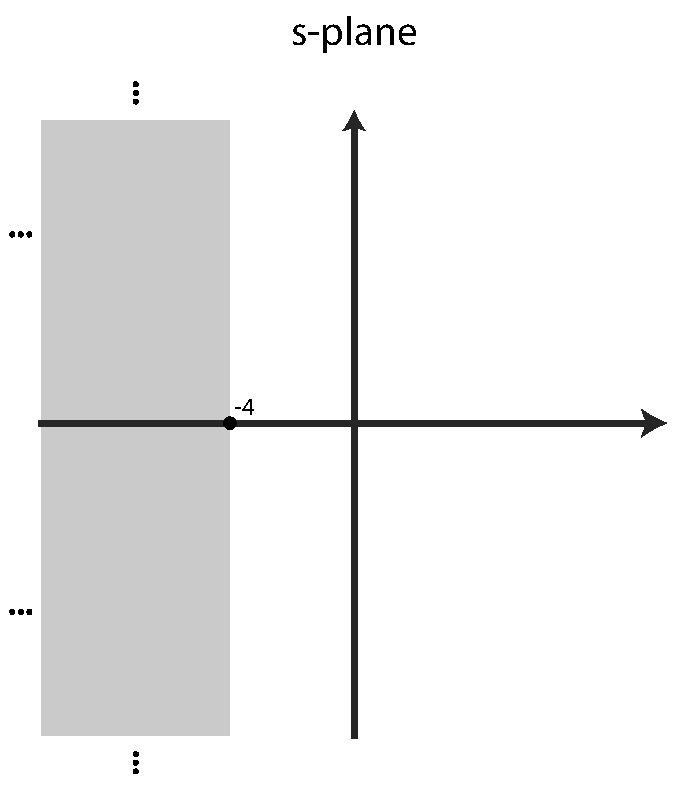
\includegraphics[width=0.4\textwidth]{settling}
    \end{center}
  \end{minipage}

We can still use Routh Hurwitz test to compute the 
$\#$ poles for which real parts is lower than $-4$.
However, we need to perform a change of variables.

Replace $s$ with $z - 4$
%
\begin{align*}
  D(s)|_{s = z- 4} = D(z)
\end{align*}
%
If we apply a Routh Hurwitz test on $D(z)$, we compute the $\#$
poles of $D(z)$ with positive real parts. Based on change of
variables, we defined 
%
\begin{align*}
\mathrm{If} \ \mathrm{Re} \lbrace z_i \rbrace > 0 \Leftrightarrow
\mathrm{Re} \lbrace s_i \rbrace > -4
\end{align*}
%
where $z_i$ and $s_i$ are poles in assocated planes. 

\vspace{12pt}

\textbf{Ex:} Let $D(s) = s^3 + 8 s^2 + 19 s + 12$, first test if the
system is BIBO stable using Routh Hurwitz test. If the system is BIBO 
stable, then check if the real parts of all the poles are located in the
region $\sigma \in (-\infty , -2)$.

\textbf{Solution:} First test the absolute stability using Routh test
on $D(s)$

\vspace{6pt}
\begin{minipage}[h]{1\linewidth}
\begin{center}
\begin{tabular}{|c || c || c  |}
\hline
$s^3$ & 1 & 19
\\ \hline
$s^2$ & 8 & 12
\\ \hline
$s^1$ & 17.5 & 0 
\\ \hline
$s^0$ & 12 & 0  
\\ \hline
\end{tabular}
\end{center}
\end{minipage}
\vspace{6pt}

Since all of the coefficients of the Routh table are positive, the
system is BIBO stable. Now check the relative stability by applying
Routh test on  ``$D(z) = D(s)|_{s = z - 2} =  z^3 + 2 z^2 - z - 2$'',

\vspace{6pt}
\begin{minipage}[h]{1\linewidth}
\begin{center}
\begin{tabular}{|c || c || c | l |}
\hline
$s^3$ & 1 & -1 & 
\\ \hline
$s^2$ & 2 & -2 & $\rightarrow A(z) = 2 z^2 - 2$
\\ \hline
$s^1$ & 4 & 0 & $\leftarrow A'(z) = 4 $
\\ \hline
$s^0$ & -2 & 0 &
\\ \hline
\end{tabular}
\end{center}
\end{minipage}
\vspace{6pt}

Since in the Routh table (with Auxiliary polynomial), there exist one
sign change, $D(z)$ has one pole in the open right half z-plane.
This means that $D(s)$ has a single pole where its real part is 
located in the $\sigma \in (-2 , 0)$ region.

If we compute the roots of $D(s)$ numerically, we find that
$p_1 = -4$, $p_2 = -3$, and $p_3 = -1$. This verifies that
the system is BIBO stable but, only two of the poles are located
in the $\sigma \in (-\infty , -2)$ region.  

\textbf{Ex:} Consider the closed-loop system that we analyzed
previously in terms of absolute stability. 

  \begin{minipage}[h]{1\linewidth}
    \begin{center}
      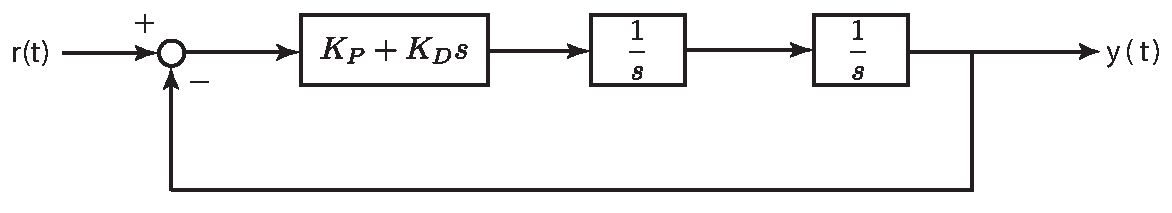
\includegraphics[width=0.75\textwidth]{example2}
    \end{center}
  \end{minipage}

Now let's fix $K_P = 20$, and find the 
set of $K_D$ gains such that closed-loop poles
are located in the desired (gray) region illustrated below.

  \begin{minipage}[h]{1\linewidth}
    \begin{center}
      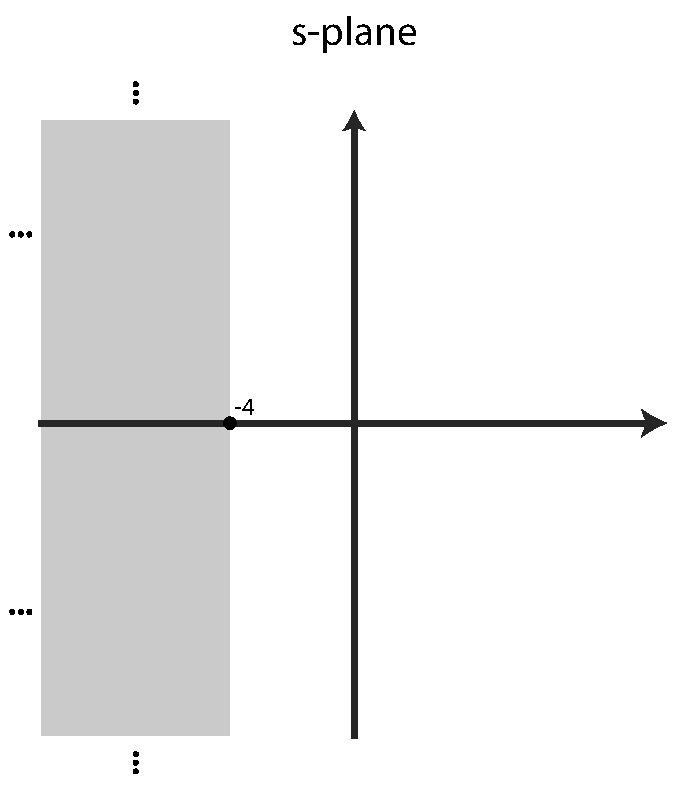
\includegraphics[width=0.4\textwidth]{settling}
    \end{center}
  \end{minipage}

\textbf{Solution:}

We can use Routh Hurwitz test on 
%
\begin{align*}
  D(z)  &= D(s)|_{s = z- 4} = (z-4)^2 + K_D (z-4) + 20
\\
&=  z^2 + (K_D - 8) z + (36 - 4 K_D)
\end{align*}
%
in order to solve this problem. 
%
\begin{table}[h]
\begin{center}
\begin{tabular}{|c || c || c  |}
\hline
$s^2$ & 1 & $36- 4 K_D$ 
\\ \hline
$s^1$ & $K_D - 8$ & 0 
\\ \hline
$s^0$ & $36- 4 K_D$ & 0 
\\ \hline
\end{tabular}
\end{center}
\end{table}
%
In order to achieve the desired pole locations, $D(z)$
can not have any poles with positive real parts, thus
the coefficients of the Routh array has to be positive.
%
\begin{align*}
  K_D > 8
  \\
  K_D < 9
\end{align*}
%
In conclusion, desired pole locations require that 
$K_D \in (8 , 9)$.



% **** This ENDS THE EXAMPLES. DON'T DELETE THE FOLLOWING LINE:
\end{document}